\documentclass[UTF8, 11pt, fontset=none]{ctexart}
\setCJKmainfont{Source Han Serif SC}
\usepackage[T1]{fontenc}

\setCJKmonofont{Source Han Mono SC}
\usepackage{underscore}

\pagestyle{plain}
\ctexset{section/format=\Large\bfseries}
\usepackage[a4paper, hmargin=1.5cm, vmargin=1.9cm]{geometry}
\setlength{\parskip}{0.5em}
\usepackage{enumitem}
\setlist{topsep=0pt,itemsep=-4pt}

\usepackage{amsmath}
\usepackage{amssymb}
\usepackage[separate-uncertainty=true]{siunitx}[=v2]

\usepackage{multirow}
\usepackage{diagbox}

\usepackage[pdfusetitle, colorlinks, urlcolor=blue, linkcolor=black]{hyperref}
\usepackage{graphicx}
\usepackage{float}
\usepackage{cleveref}
\crefname{figure}{图}{图}
\crefname{table}{表}{表}
\crefname{page}{页}{页}
\crefname{section}{节}{节}

\usepackage[normalem]{ulem}

\begin{document}

\title{数字逻辑设计 12 组(Chrome 小恐龙)实验报告}
\author{致理-信计 11 \hspace{2pt} 游宇凡 \hspace{12pt} 计14 \hspace{2pt} 王博文}
\maketitle

\section{项目介绍}

《恐龙游戏》(英语:Dinosaur Game)是一款内置于 Google Chrome 的网页游戏,会在用户断网时自动出现,也可以通过访问 \texttt{chrome://dino} 来游玩。玩家在横向滚动栏形式的恐龙游戏中,操控一只像素风格的小暴龙跳跃、下蹲以避开障碍物并获取分数。

\begin{figure}[H]
    \centering
    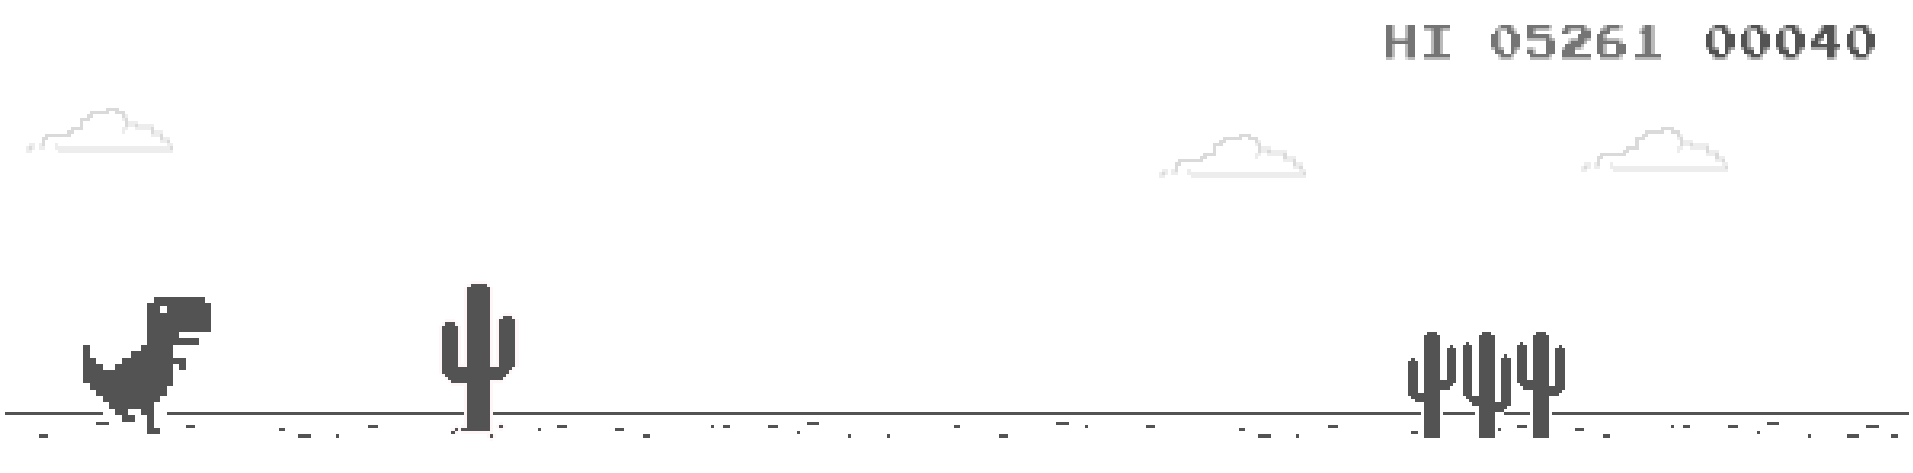
\includegraphics[width=\textwidth]{images/cover.png}
    \caption{Chrome 恐龙游戏截图}
    \label{cover}
\end{figure}

我们使用 FPGA 复刻这一游戏,支持按键和传感器两种输入方式,并使用 VGA 输出。使用传感器时,需要玩家将传感器绑在大腿上,传感器将检测玩家跳跃和下蹲的动作,在增加趣味性的同时,还能起到一定的健身作用。\scriptsize\sout{(测试的时候跳得确实很累)}\normalsize

\section{总体设计}

\subsection{模块总体划分和分工}

总体设计分为传感器模块、画面输出模块和游戏逻辑模块。

我们的分工非常简明,由游宇凡同学负责传感器(外设组装调试以及代码编写)和画面输出,由王博文同学负责游戏逻辑。两位同学所负责模块之间的接口也非常简单,只有蹲下、起跳的信号,画面上每个元素的坐标信息,控制昼夜转换的信号,以及画面刷新信号、时钟信号等,这大大降低了我们的沟通成本。

\subsection{文件说明}

\begin{table}[H]
    \centering
    \caption{文件说明}
    \vspace{1em}
    \small
    \begin{tabular}{|c|c|c|c|}
        \hline
        目录 & 文件名 & 描述 & 主要完成者 \\
        \hline
        \multirow{20}*{\texttt{src}}
            & \texttt{async_receiver.sv} & 接收 UART 数据 & 游宇凡 \\ \cline{2-4}
            & \texttt{cloud.sv} &  & 王博文 \\ \cline{2-4}
            & \texttt{distance_meter.sv} &  & 王博文 \\ \cline{2-4}
            & \texttt{dpy_scan.v} & 实验板上的数码管显示 & 助教(即提供的代码模板) \\ \cline{2-4}
            & \texttt{horizon.sv} &  & 王博文 \\ \cline{2-4}
            & \texttt{horizon_line.sv} &  & 王博文 \\ \cline{2-4}
            & \texttt{mod_top.sv} & 顶层模块 & 游宇凡、王博文、助教 \\ \cline{2-4}
            & \texttt{motion_detector.sv} & 由传感器数据判断运动状态 & 游宇凡 \\ \cline{2-4}
            & \texttt{obstacle.sv} &  & 王博文 \\ \cline{2-4}
            & \texttt{painter.sv} & 逐个绘制背景和画面元素 & 游宇凡 \\ \cline{2-4}
            & \texttt{paint_background.sv} & 绘制画面背景 & 游宇凡 \\ \cline{2-4}
            & \texttt{paint_element.sv} & 绘制单个画面元素 & 游宇凡 \\ \cline{2-4}
            & \texttt{palette.sv} & 由颜色编号以及昼夜转换获取 RGB 值 & 游宇凡 \\ \cline{2-4}
            & \texttt{resetter.sv} & 启动时自动复位,之后按按钮复位 & 游宇凡、王博文 \\ \cline{2-4}
            & \texttt{runner.sv} &  & 王博文 \\ \cline{2-4}
            & \texttt{sensor.sv} & 解析传感器数据 & 游宇凡 \\ \cline{2-4}
            & \texttt{spike_filter.sv} & 信号消抖(用于 UART) & 游宇凡 \\ \cline{2-4}
            & \texttt{synchronizer.sv} & 异步信号同步化(用于 UART) & 游宇凡 \\ \cline{2-4}
            & \texttt{trex.sv} &  & 王博文 \\ \cline{2-4}
            & \texttt{vga.sv} & 显存 \& VGA 输出 & 游宇凡、助教 \\ \hline
        \multirow{7}*{\texttt{src/sim}}
            & \texttt{async_receiver_sim.sv} & \multirow{7}*{相应模块的仿真测试} & 游宇凡 \\ \cline{2-2} \cline{4-4}
            & \texttt{distance_meter_sim.sv} & & 王博文 \\ \cline{2-2} \cline{4-4}
            & \texttt{horizon_sim.sv} & & 王博文 \\ \cline{2-2} \cline{4-4}
            & \texttt{obstacle_sim.sv} & & 王博文 \\ \cline{2-2} \cline{4-4}
            & \texttt{runner_sim.sv} & & 王博文 \\ \cline{2-2} \cline{4-4}
            & \texttt{sensor_sim.sv} & & 游宇凡 \\ \cline{2-2} \cline{4-4}
            & \texttt{trex_sim.sv} & & 王博文 \\ \hline
        \multirow{4}*{\texttt{src/util}}
            & \texttt{collision.sv} &  & 王博文 \\ \cline{2-4}
            & \texttt{lfsr.v} &  &  \\ \cline{2-4}
            & \texttt{lfsr_prng.sv} &  & \\ \cline{2-4}
            & \texttt{util_func.sv} &  & 王博文 \\ \hline
        \texttt{tools} & \texttt{image-to-mif.py} & 将图片转换为 MIF 文件(2 bit 字宽) & 游宇凡 \\ \hline
        \multirow{3}*{\texttt{assets}}
            & \texttt{sprite.xcf} & \multirow{2}*{将原版 sprite 图的压缩至四种颜色} & Chromium、游宇凡 \\ \cline{2-2} \cline{4-4}
            & \texttt{sprite.png} & & 由 GIMP 生成 \\ \cline{2-4}
            & \texttt{sprite.mif} & 存于 ROM 中的 sprite 图 & 由 \texttt{image-to-mif.py} 生成 \\ \hline
    \end{tabular}
    \normalsize
    \label{file-description}
\end{table}

\section{模块设计}

\subsection{传感器模块}

\subsubsection{外设}

采用一个 JY901S 运动姿态传感器测量玩家的运动数据,以及一对 HC-12 无线模块来向实验板传输数据,波特率设为 \SI{57600}{bps}。元件之间直接焊接相连,固定在面包板上,由充电宝和 USB 转 TTL 模块进行供电,整体粘在为 Switch 健身环设计的绑腿上。

\subsubsection{代码}

参考 \href{https://www.fpga4fun.com/SerialInterface.html}{fpga4fun - Serial interface} 编写了 UART 数据接收,参考 \href{https://wit-motion.yuque.com/wumwnr/ltst03/vl3tpy}{WIT 私有协议} 使用状态机逐字节接受数据并解析。

采用简单的阈值判断来检测玩家起跳/下蹲的动作:与水平方向夹角小于 \SI{56.25}{\degree} 则判断为下蹲,竖直方向加速度达到向下 $0.75g$(这里是转换为了实际运动的加速度,原始测量值则是大于 $-0.25g$)则判断为起跳。

\subsection{画面输出模块}

图像的绘制基于原版恐龙游戏使用的 \href{https://github.com/chromium/chromium/blob/3b31f1cbd28e0a1199defe6f6b37001cef4c4790/components/neterror/resources/images/default_200_percent/offline/200-offline-sprite.png}{sprite 图},采用 \href{http://tinyvga.com/vga-timing/1280x800@60Hz}{1280$\times$800 @ 60Hz} 的分辨率,其中 1280$\times$300 的部分是实际游戏画面,和原版画面大小大致相同,剩下的部分是空白。

\subsubsection{显存 \& VGA 输出}

采用双显存机制,将片内 RAM 的一半用于写入,一半用于读取,每帧对两块显存进行交换。通过 ring buffer 修复读取缓存产生的延时导致的像素偏移。显存采用 \SI{33.33}{\mega\hertz} 的写入时钟和 VGA 所需的 \SI{83.46}{\mega\hertz} 读取时钟。VGA 模块提供一个画面刷新信号输出,用来告诉游戏逻辑模块需要更新画面。VGA 模块还接受黑夜程度作为输入以实现昼夜转换,为了支持渐变还需要得到过程中的颜色值,如果直接进行乘法运算会有较大的延时,难以在 VGA 的高频时钟下完成计算,所以实际采用的方案是在编译时就计算出所有可能的颜色值(具体实现为使用 $0 \sim 255$ 作为 \texttt{parameter} 分别进行实例化),根据黑夜程度进行选择。

\subsubsection{元素绘制}

sprite 图转为 MIF 文件存在片内 ROM 中,原版 sprite 共有 17 种颜色,通过 GIMP 压缩至只有 4 种颜色,使得 ROM 和显存中每个像素只占据 2 个 bit,从而可以放进 FPGA 的内置存储资源(共使用 $2446 \times 194 \times 2 + 2 \times 1280 \times 300 \times 2 \approx \SI{2.49}{\mega b}$ 存储资源)。元素绘制模块接受 sprite 坐标、画面绘制坐标、元素宽高作为参数,从 ROM 中读取每个像素,通过状态机依次绘制空白背景和每个元素。

\subsection{游戏逻辑模块}

\section{仿真结果}

\section{实验演示说明}

\subsection{实验板输入}

两个带去抖按键中,左边的是复位,右边的是跳跃以及开始/重启游戏。四个普通按键中位于右下的是下蹲。16 位拨码开关中最右边的用于控制输入方式,ON 是按键输入,OFF 是传感器输入。

实验板一侧的无线模块直接插在 Pmod 1 的 $2 \sim 6$ 引脚,方向由 VCC 和 GND 确定。

\subsection{传感器使用}

将传感器绑在大腿上,接线的一侧竖直向上,将 USB 转 TTL 模块插入充电宝供电,充电宝放在口袋中或拿在手上。

\section{遇到的问题及解决}

\subsection{外设组装遇到的问题}

一开始我们打算使用面包板进行连线和固定,使用纽扣电池(\SI{6}{\volt} 电池盒 + \SI{3.3}{\volt} 稳压模块)进行供电。

最先遇到的问题是排针没有焊接,导致接触非常不良,几乎完全不可用,焊接后就好了很多。

调试时,先是将无线模块连到电脑上通过无线模块和传感器附带的软件进行调试,这需要使用 USB 转 TTL 模块来与电脑连接。一开始是使用实验板为无线模块供电,就忘了和 USB 转 TTL 模块共地,导致读不到数据。实际上,除了将 USB 转 TTL 模块与实验板共地,更简单的做法是直接通过 USB 转 TTL 模块来为无线模块供电。

使用纽扣电池时,观察到数据传输速率很慢,而且经常过几十秒就完全停止了。经过一系列的排查,最终确定了问题在于纽扣电池的电流太小,无法带动传感器和无线模块。尝试过调整无线模块的工作模式来降低工作电流,情况略有好转但仍然不是很好。于是只能放弃使用纽扣电池供电,改用充电宝供电,之前为了调试购买的 USB 转 TTL 模块刚好可以用来供电。

连到实验板上时还遇到了一个小问题:Pmod 接口的引脚编号和 IO 引脚的序号是不同的,1、2、3、4、7、8、9、10 号引脚分别是 IO0 $\sim$ IO7,一开始没看清导致引脚绑定偏了一位。

这时,外设整体的连接依然不是很稳定,跳几下之后就很容易断开连接,用手稍微按压一下线又会恢复工作。尝试过用透明胶对整体进行固定,有一定的效果,但仍不理想,而且过了几天后可能反而会整体全部松动,需要将胶带拆开才能调整修复。最后改成了所有连线都焊上,连接就非常稳定了。

\subsection{传感器跳跃检测遇到的问题}

一次典型的跳跃的加速度曲线如\cref{sensor-jump} 所示,一开始先略微上升是在下蹲,后来的一段下降是在加速起跳,后面上升至 0 附近是腾空时接近失重状态,落地时有一个猛烈的下降。

\begin{figure}[ht]
    \centering
    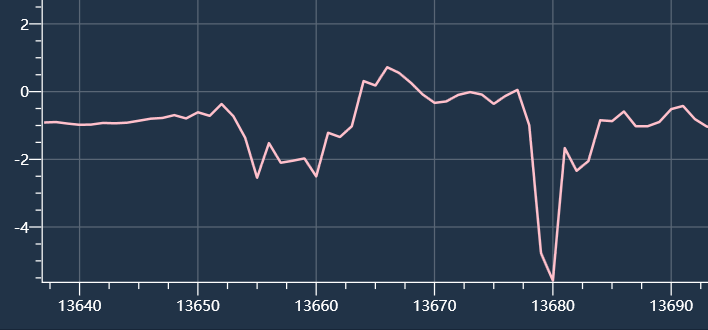
\includegraphics[width=0.8\textwidth]{images/sensor-jump.png}
    \caption{跳跃时传感器检测到的加速度曲线}
    \label{sensor-jump}
\end{figure}

最终采用的阈值判断本质上是在检测腾空的这一段,这导致检测到的时机略晚于起跳,会让玩家感到一定的延迟,影响游戏体验,所以我们尝试了多种方法来试图优化跳跃检测的灵敏性、准确性和即时性。但最后这些方法都没有取得更好的效果,只能退而求其次,通过给玩家多条生命来缓解游戏难度过高带来的问题。

\subsubsection{对加速度积分得到速度}

仅检测加速度是不太准确的,如果能检测速度就会好很多。但是简单地积分会产生严重的累积误差,传感器的时间粒度也不够细,而且传感器检测到的不是实际运动的加速度,而是带 $g$ 的加速度,为了得到实际运动的加速度就需要得到 $g$ 的值,而 $g$ 的误差又会带来更严重的累积误差。所以我们最终放弃了这一方案。

\subsubsection{检测全方位总加速度而非竖直方向加速度}

因为本质上是在检测腾空的这一段,而腾空时近似处于失重状态,其实可以不止检测竖直方向加速度,而是检测总加速度,总加速度(的绝对值)足够小就可以视为是腾空,这样的话可以一定程度上避免下蹲之类的动作被误识别为腾空,从而允许设置更宽松的阈值。这个思路应该是没有太大问题的,但实际测试时发现效果和之前差不多甚至略差。一个可能的解释:从\cref{sensor-jump} 中可以看出,腾空最开始时有一段加速度远超 $0$,判断竖直方向加速度时只需判断加速度大于一个负数,判断总加速度时则是判断加速度绝对值小于一个数,这会导致过大的加速度被漏判。

\subsubsection{检测起跳而非腾空}

检测腾空不可避免地会有一定的延迟,但检测起跳的主要问题在于,起跳和落地的加速度曲线是类似的,需要想办法进行区分。

起跳的持续时间往往比落地长,但持续时间会因玩家动作而有较大的变化,如果检测起跳的持续时间,一方面可能造成误判、漏判,另一方面也会导致检测不及时。

还有一个思路是在检测到腾空后的短时间内禁用跳跃检测,但这样在理论上就会有连跳被漏判的风险,实际测试时效果也非常不好。

\subsection{画面输出遇到的问题}

在存 sprite 图时,一开始使用的是 \href{https://github.com/thu-cs-lab/MifConverter}{MifConverter},得到的 MIF 文件字宽不对,而 MifConverter 只支持 8 的倍数的字宽,所以自己写了一个脚本来进行转换。

为了避免出现时序问题,需要降低元素绘制使用的时钟频率,但为了在一帧内完成显存的写入,至少需要 $1280 \times 300 \times 60 \times (1+\alpha)$ 的时钟频率,其中 $\alpha$ 表示画面上所有元素的 bounding rectangle 大小之和占画面总大小的比例。最终我们选择了使用 \SI{33.33}{\mega\hertz} 的时钟,这允许大约 \SI{40}{\percent} 的画面元素占比。

在信号跨时钟域时如果不处理好也会出现时序问题,最简单且可靠的处理方式是使用一个写入时钟和读取时钟不同的只存 1 bit 数据的 RAM IP 核。

除了降低时钟频率,也需要避免使用组合逻辑进行输出,可以加一个 buffer。

\end{document}
